\newpage
\tikz[remember picture,overlay] \node[opacity=1,inner sep=0pt] at (current page.center){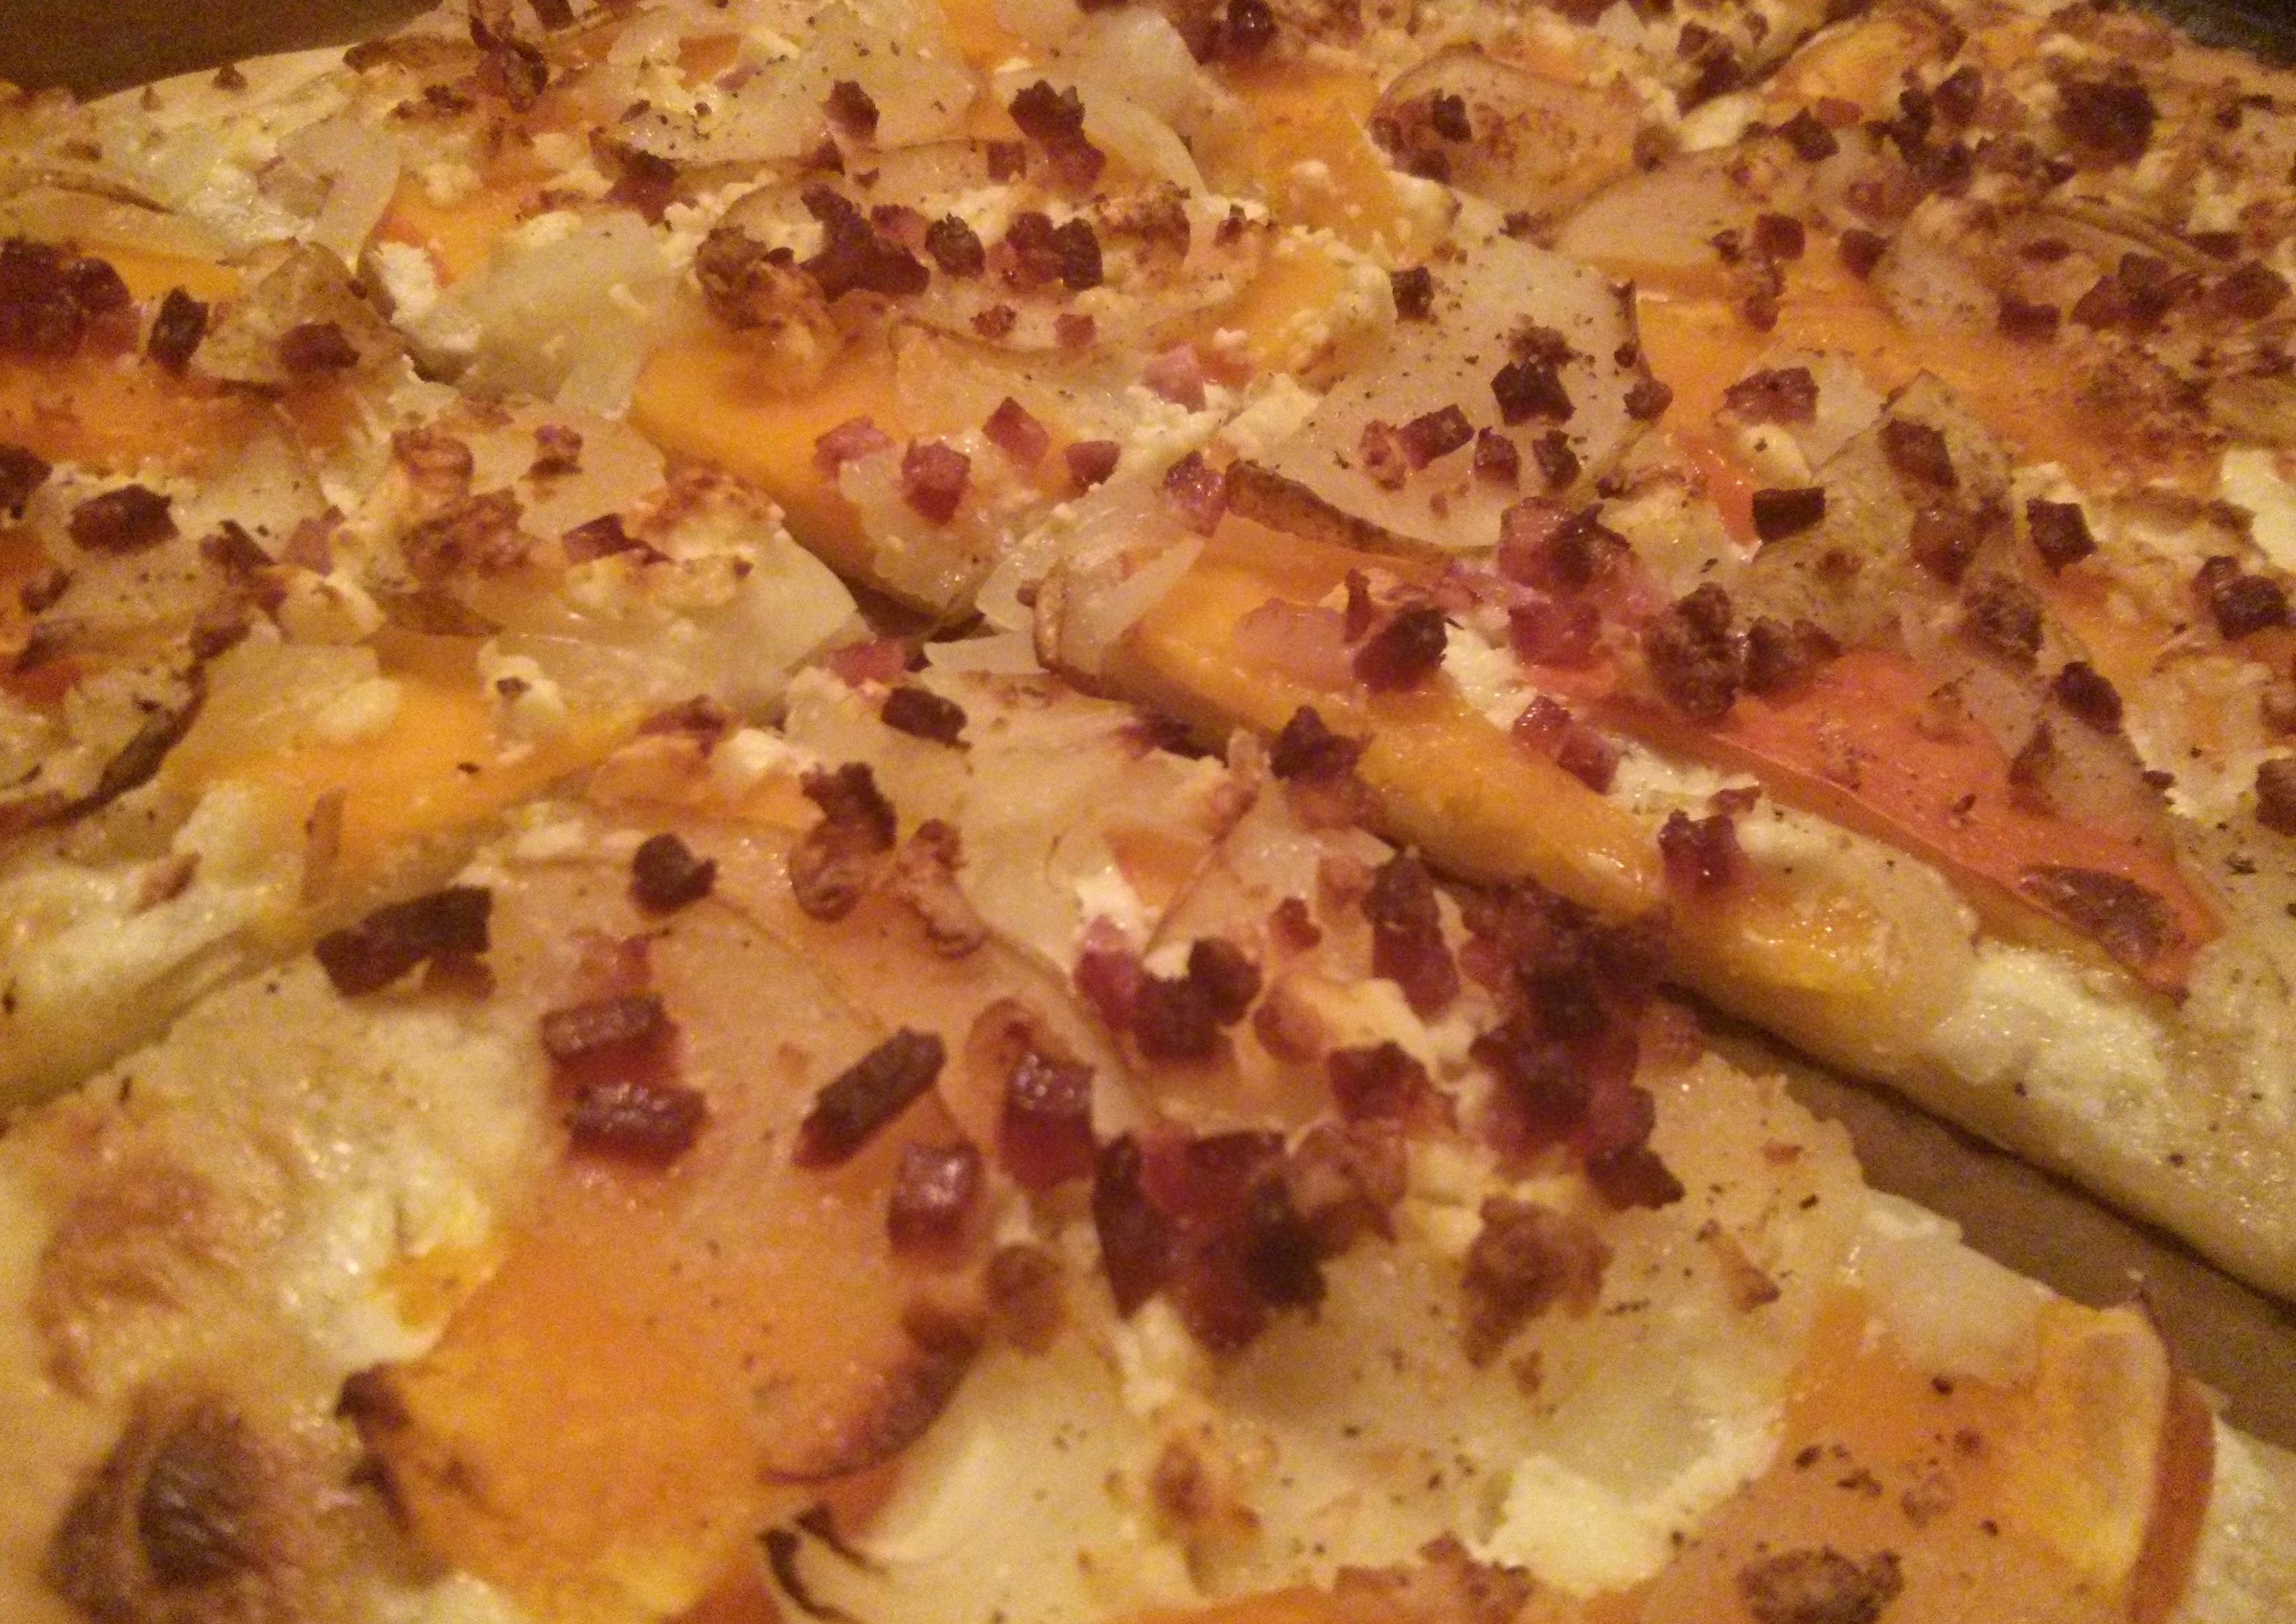
\includegraphics[width=\paperwidth,height=\paperheight]{./bilder/kuerbis_flammkuchen_ratio.jpg}};

\begin{recipe}[]{Kürbis-Flammkuchen} %Quelle
	\timerecipe[Minuten]{ca. 10+30} %mit [EINHEIT]
	\personcount[Blech]{1} % mit[ART]
	\ingredient{350g Mehl} % ggf. \nicefrac{1}{2}
	\ingredient{0,5 TL Zucker}
	\ingredient{0,5 TL Salz}
	\ingredient{3 EL Olivenöl}
	\ingredient{175ml Wasser}
	\ingredient{250g Hokkaidokürbis}
	\ingredient{1 große Zwiebel}
	\ingredient{100g Speckwürfel}
	\ingredient{1 Birne}
	\ingredient{200g Schmand}
	\ingredient{1 Feta}


\step
\textbf{350g Mehl}, \textbf{0,5 TL Zucker}, \textbf{0,5 TL Salz}, \textbf{3 EL Olivenöl} und \textbf{175ml Wasser} zu einem Teig kneten.

\step
\textbf{1 Zwiebel} in Ringe schneiden, \textbf{250g Hokkaidokürbis} in 0,5cm dicke Scheiben schneiden, \textbf{1 Birne} in Spalten schneiden und \textbf{1 Feta} in Würfel schneiden.

\step
Teig ausrollen, mit \textbf{200g Schmand} bestreichen, mit \textbf{Salz} und \textbf{Pfeffer} würzen und mit \textbf{100g Speckwürfeln}, den Kürbisschnitzen, den Birnenspalten, den Fetawürfeln und den Zwiebelringen belegen.

\step 
Ca. 25 Minuten bei 250°C (230°C Umluft) backen.

%\tippbox{\textbf{Tipp:} ...} % Tipp in extra Rahmen
\end{recipe}